\section{Supplementary empirical displays}
\label{app:displays}
All displays use the same measured results as Section~\ref{sec:results}. Their captions identify each cohort and intervention. Full-gain common-challenger comparisons exclude the union of incumbent winners; task-composition and random-selection summaries use the full evaluation cohorts. Neither geometric means nor medians silently replace missing or zero scores. Figure/table generators and input/output mappings are recorded in \texttt{presentation/manifest.json} and \texttt{presentation/README.md}.

\begin{table}[htbp]
\caption{\CohortsCaption}
\label{tab:cohorts}
\centering\small
\input{tables/cohorts}
\end{table}
\begin{table}[htbp]
\caption{\PairedBordaCaption}
\label{tab:paired}
\centering\small
\input{tables/paired_borda}
\end{table}
\begin{table}[htbp]
\caption{\CeilingSensitivityCaption}
\label{tab:ceiling}
\centering\small
% Generated by presentation/render.py; do not edit numerical entries.
\begin{tabular}{lrrrr}
\toprule
Rule & HELM unit & HELM observed & Open unit & Open observed \\
\midrule
Mean & 16 & 37 & 2 & 4 \\
Median & 21 & 21 & 3 & 3 \\
Geometric & 16 & 36 & 3 & 5 \\
Minimum & 12 & 12 & 3 & 3 \\
Borda & 48 & 49 & 6 & 6 \\
\bottomrule
\end{tabular}

\end{table}
\begin{table}[htbp]
\caption{\RandomSelectionCaption}
\label{tab:random}
\centering\small
\input{tables/random_selection}
\end{table}
\begin{table}[htbp]
\caption{\RobustnessCaption}
\label{tab:robustness}
\centering\small
\input{tables/robustness}
\end{table}
\begin{figure}[htbp]
\centering
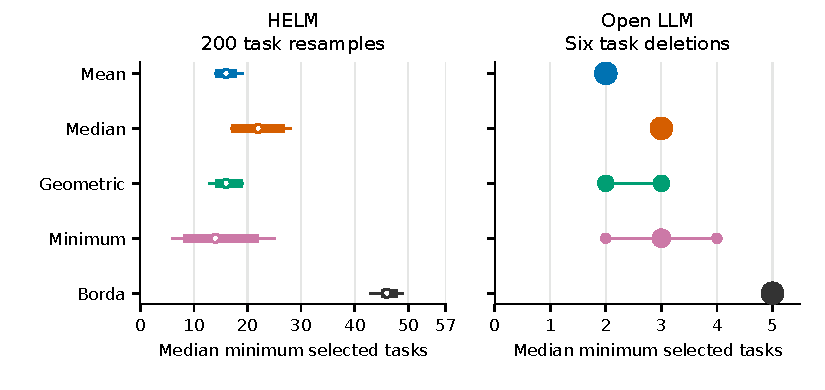
\includegraphics[width=\linewidth]{figures/task_composition.pdf}
\caption{\TaskCompositionCaption}
\label{fig:composition}
\end{figure}
\clearpage
